%% \newcommand{\paperfilebase}{/Users/andyreagan/projects/2014/09-books/media/overleaf-git/emotional-arcs}
\chapter{Selected contributions to published work}
\chaptermark{Contributions} %this is the chapter heading that will show on subsequent pages
\label{chap:contributions}

Throughout the course of my studies at the University of Vermont,
I have enjoyed the collaborative research environment
afforded by the Computational Story Lab \footnote{In this Chapter I use the singular first person noun in place of the plural pronoun to discuss my individual contributions}.
As a result of these collaborations, I have assisted in the preparation of 10 other research papers.
I have variously done data visualization work, curated data from our Twitter database, built interactive online appendices, and assisted in performing mathematical analysis.
In this Chapter, I detail my contributions to each of these 10 papers, beginning with the paper abstract and then discussing my personal contribution.

%% \begin{quote}
%% \input{\paperfilebase.abs}
%% \end{quote}

\pagebreak

\section{Collective Philanthropy: Describing and Modeling the Ecology of Giving}

The first paper is \textit{Collective Philanthropy: Describing and Modeling the Ecology of Giving} by William L. Gottesman, Andrew James Reagan, and Peter Sheridan Dodds, cited as \cite{gottesman2014collective}.

\subsection{Abstract}
\begin{quote}
  Reflective of income and wealth distributions,
  philanthropic gifting appears to follow an approximate power-law size distribution as measured by the size of gifts received by individual institutions.
We explore the ecology of gifting by analyzing data sets of individual gifts for a diverse group of institutions dedicated to education, medicine, art, public support, and religion.
We find that the detailed forms of gift-size distributions differ across but are relatively constant within charity categories.
We construct a model for how a donor's income affects their giving preferences in different charity categories, offering a mechanistic explanation for variations in institutional gift-size distributions.
We discuss how knowledge of gift-sized distributions may be used to assess an institution's gift-giving profile, to help set fund-raising goals, and to design an institution-specific giving pyramid.
\end{quote}

\subsection{Contribution}

In this paper I prepared final versions of each visualization in the paper, working from the initial designs from both Professor Dodds and Bill Gottesman, and working closely with Professor Dodds in their preparation.
Additionally and at the request of the reviewers, I performed the statistical tests for support of power law distributions discussed in the paper, and included in the Appendix.
In addition to testing for support of power law distributions using the MLE estimator \cite{clauset2009b}, I ran likelihood comparison tests across many distributions, which we argue in the manuscript are potentially more applicable here to determine the most appropriate distribution.
The parameters for the various distributions mentioned in the paper are written using LaTeX variables, written in a .tex file by the MATLAB and Python scripts that perform the statistical procedures.
To the extent possible, all figures and analysis can be reproduced by running a single script.
In this Section we include a reprint of Figure 1, Figure S1, and the power law fit tables from the paper.
The codebase for creating the figures and performing the statistical procedures is available at \href{https://github.com/andyreagan/philanthropy-distributions-code}{https://github.com/andyreagan/philanthropy-distributions-code}.

\begin{figure}[tbp!]
  \centering
  \includegraphics[width=0.96\textwidth]{/Users/andyreagan/projects/2012/01-philanthropy-distributions/figures/local/figphdists001_noname.pdf}
  \caption[]{
    A reprint of Figure 1 from \cite{gottesman2014collective}, part of the caption is as follows:
    ``Gift size distributions for a range of institutions.
    The reported $\alpha$ and $\gamma$ were fitted to the region
indicated by solid gray line, and the 95\% CI of this fit, as well as
year for which the fit is plotted, are included for each organization.
    The ranges over which the data were fit was chosen empirically; other approaches were found to be inconsistent (see Supplementary).''
      }
  \label{fig:philanthropy-001}
\end{figure}

\begin{figure}[tbp!]
  \centering
  \includegraphics[width=0.96\textwidth]{/Users/andyreagan/projects/2012/01-philanthropy-distributions/figures/local/KSvsXmin_inst_4_noname.pdf}
  \caption[]{
    A reprint of Figure S1 from \cite{gottesman2014collective}, part of the caption is as follows:
    ``The Kolmogorov-Smirnoff statistic $D$ plotted over the log of $x_{\min}$, the minimum value fit for power law behavior, for the United Way of Chittenden County over the years 2006-2010.
    $D$ is generated from the ML estimate.
    Existence of multiple minima in our data indicate that there are multiple possible fitting regions for which the KS statistic details a good fit.
    The variability of this value over each year plotted produced widely varying scaling parameters $\gamma$, and thus cannot be used without actually looking at the data.''
      }
  \label{fig:philanthropy-S001}
\end{figure}

{\scriptsize
\input{/Users/andyreagan/projects/2012/01-philanthropy-distributions/philanthropy-distributions.supplementary-inst-sideways}
}

\pagebreak
\clearpage

\section{Shadow networks: Discovering hidden nodes with models of information flow}

Paper number two is \textit{Shadow networks: Discovering hidden nodes with models of information flow} by James P. Bagrow, Suma Desu, Morgan R. Frank, Narine Manukyan, Lewis Mitchell, Andrew Reagan, Eric E. Bloedorn, Lashon B. Booker, Luther K. Branting, Michael J. Smith, Brian F. Tivnan, Christopher M. Danforth, Peter S. Dodds, and Joshua C. Bongard, cited as \cite{bagrow2014shadow}.

\subsection{Abstract}
\begin{quote}
  %% James P. Bagrow, Suma Desu, Morgan R. Frank, Narine Manukyan, Lewis Mitchell, Andrew Reagan, Eric E. Bloedorn, Lashon B. Booker, Luther K. Branting, Michael J. Smith, Brian F. Tivnan, Christopher M. Danforth, Peter S. Dodds, Joshua C. Bongard
  Complex, dynamic networks underlie many systems, and understanding these networks is the concern of a great span of important scientific and engineering problems.
  Quantitative description is crucial for this understanding yet, due to a range of measurement problems, many real network datasets are incomplete.
Here we explore how accidentally missing or deliberately hidden nodes may be detected in networks by the effect of their absence on predictions of the speed with which information flows through the network.
We use Symbolic Regression (SR) to learn models relating information flow to network topology.
  These models show localized, systematic, and non-random discrepancies when applied to test networks with intentionally masked nodes, demonstrating the ability to detect the presence of missing nodes and where in the network those nodes are likely to reside.
\end{quote}

\subsection{Contribution}

This paper is the result of a multi-day intensive collaboration called a Flash Mob Research Event.
The format is one or two days of everyone in the same room, brain storming how to tackle an important open question.
An outline of the paper is written, and after the event each member works to complete their part in carrying out the research idea.
My responsibility was to build reciprocal reply networks from Twitter data, in an effort to measure information flow over the network.
The network construction proceeded in three steps: (1) build a network using replies, (2) measure information flow over this reciprocal reply network, and (3) collect edges in the network for the actual information flow.
Each step of the construction would be carried out over a number of days, and using a single node on the VACC, we were able to build networks in memory for a total of 9 days.
These 9 days were considered for combinations of 3/3/3 or 4/4/1 days, respectively.
These data were used in a real world test, to accompany testing of simulated data.

\section{Human language reveals a universal positivity bias}

Paper number three is \textit{Human language reveals a universal positivity bias} by Peter Sheridan Dodds, Eric M. Clark, Suma Desu, Morgan R. Frank, Andrew J. Reagan, Jake Ryland Williams, Lewis Mitchell, Kameron Decker Harris, Isabel M. Kloumann, James P. Bagrow, Karine Megerdoomian, Matthew T. McMahon, Brian F. Tivnan, and Christopher M. Danforth, cited as \cite{dodds2015human}.

\subsection{Abstract}
\begin{quote}
  %% Peter Sheridan Dodds, Eric M. Clark, Suma Desu, Morgan R. Frank, Andrew J. Reagan, Jake Ryland Williams, Lewis Mitchell, Kameron Decker Harris, Isabel M. Kloumann, James P. Bagrow, Karine Megerdoomian, Matthew T. McMahon, Brian F. Tivnan, Christopher M. Danforth
  Using human evaluation of 100,000 words spread across 24 corpora in 10 languages diverse in origin and culture, we present evidence of a deep imprint of human sociality in language, observing that
  (1) the words of natural human language possess a universal positivity bias;
  (2) the estimated emotional content of words is consistent between languages under translation;
  and (3) this positivity bias is strongly independent of frequency of word usage.
  Alongside these general regularities, we describe inter-language variations in the emotional spectrum of languages which allow us to rank corpora.
We also show how our word evaluations can be used to construct physical-like instruments for both real-time and offline measurement of the emotional content of large-scale texts.
\end{quote}

\subsection{Contribution}

In this paper I built the online appendices and performed additional tests of our method for building the sentiment timeseries for books (measuring their emotional arcs).
This included building a fully interactive version of an application of this dataset to analyze the emotional arcs of stories, which was done for a selection of the Western Canon and Project Gutenberg books.
In particular, we analyzed the emotional arc for these books in their original language, providing translations of the word shifts graphs into English.
The translations relied upon the translations of Google Translate, as curated by Eric Clark.
The additional statistical tests amounted to randomly shuffling the words in each book which we showcased, to demonstrate that the emotional arcs were meaningful.

\section{Climate change sentiment on Twitter: An unsolicited public opinion poll}

Paper number four is \textit{Climate change sentiment on Twitter: An unsolicited public opinion poll} by Emily M. Cody, Andrew J. Reagan, Lewis Mitchell, Peter Sheridan Dodds, and Christopher M. Danforth, cited as \cite{cody2015climate}.

\subsection{Abstract}
\begin{quote}
  %% Emily M. Cody, Andrew J. Reagan, Lewis Mitchell, Peter Sheridan Dodds, Christopher M. Danforth
  The consequences of anthropogenic climate change are extensively debated through scientific papers, newspaper articles, and blogs.
Newspaper articles may lack accuracy, while the severity of findings in scientific papers may be too opaque for the public to understand.
Social media, however, is a forum where individuals of diverse backgrounds can share their thoughts and opinions.
As consumption shifts from old media to new, Twitter has become a valuable resource for analyzing current events and headline news.
In this research, we analyze tweets containing the word "climate" collected between September 2008 and July 2014.
Through use of a previously developed sentiment measurement tool called the Hedonometer, we determine how collective sentiment varies in response to climate change news, events, and natural disasters.
We find that natural disasters, climate bills, and oil-drilling can contribute to a decrease in happiness while climate rallies, a book release, and a green ideas contest can contribute to an increase in happiness.
Words uncovered by our analysis suggest that responses to climate change news are predominantly from climate change activists rather than climate change deniers, indicating that Twitter is a valuable resource for the spread of climate change awareness.
\end{quote}

\subsection{Contribution}

In this paper I was responsible for the data curation.
This amounted to searching the Twitter database on the VACC for a variety of keywords, storing those results, and processing them into useful formats for analysis.
Weighing at approximately 37TB of compressed JSON files, the Twitter database is difficult to search quickly over the GPFS architecture of the VACC, and only possible through the use of many short runtime (less than 2 hour) jobs.
Given all of this, a single search of the database takes approximately 2 days if everything is running smoothly.

\section{Reply to Garcia et al.: Common mistakes in measuring frequency dependent word characteristics}

The fifth paper is \textit{Reply to Garcia et al.: Common mistakes in measuring frequency dependent word characteristics} by P. S. Dodds, E. M. Clark, S. Desu, M. R. Frank, A. J. Reagan, J. R. Williams, L. Mitchell, K. D. Harris, I. M. Kloumann, J. P. Bagrow, K. Megerdoomian, M. T. McMahon, B. F. Tivnan, and C. M. Danforth, cited as \cite{dodds2015reply}.

\subsection{Abstract}
\begin{quote}
  %% P. S. Dodds, E. M. Clark, S. Desu, M. R. Frank, A. J. Reagan, J. R. Williams, L. Mitchell, K. D. Harris, I. M. Kloumann, J. P. Bagrow, K. Megerdoomian, M. T. McMahon, B. F. Tivnan, C. M. Danforth
  We demonstrate that the concerns expressed by Garcia et al. are misplaced, due to
  (1) a misreading of our findings in \cite{dodds2015human};
  (2) a widespread failure to examine and present words in support of asserted summary quantities based on word usage frequencies;
  and (3) a range of misconceptions about word usage frequency, word rank, and expert-constructed word lists.
In particular, we show that the English component of our study compares well statistically with two related surveys, that no survey design influence is apparent, and that estimates of measurement error do not explain the positivity biases reported in our work and that of others.
We further demonstrate that for the frequency dependence of positivity
---of which we explored the nuances in great detail in \cite{dodds2015human}
---Garcia et al did not perform a reanalysis of our data---
they instead carried out an analysis of a
statistically improper data set and introduced a nonlinearity before performing linear regression.
\end{quote}

\subsection{Contribution}

For this paper I built a new online appendix, performed tests of the claims made by Garcia \etal (including re-making their visualizations), and built visualizations for the extended version of the reply (e.g. Table I and Figure 1 in the arXiv version).
Below, we include a reprint of the aforementioned Figure 1 and reproduction of the Figure from Garcia \etal:

\begin{figure}[ht]
  \centering
  \includegraphics[width=0.96\textwidth]{/Users/andyreagan/projects/2015/03-sentiment-comparison/figures/PNAS/2015-08-16-12-53-scatter-LabMT-WK-ANEW.pdf}
  \caption[]{
    Reprint of Figure 1 from \cite{dodds2015reply}, with the caption as follows:
       ``Comparison of word ratings for three studies for
    overlapping words:
    labMT~\citep{dodds2011temporal},
    ANEW~\citep{bradley1999affective},
    and Warriner and Kuperman~\citep{warriner2013norms}
    Reduced major axis regression~\citep{rayner1985linear} yield
    the fits $\havgfn' = \beta \havgfn + \alpha$.''
  }
  \label{fig:reply-001}
\end{figure}

\begin{figure}[ht]
  \centering
  
\includegraphics[width=0.45\textwidth]{/Users/andyreagan/projects/2015/03-sentiment-comparison/figures/PNAS/reply-fig1.pdf}
  
\includegraphics[width=0.45\textwidth]{/Users/andyreagan/projects/2015/03-sentiment-comparison/figures/PNAS/warriner_fig1.pdf}
  \caption[]{
    A reproduction of the Figure 1A and 1B from \cite{garcia2015language}.
      }
  \label{fig:reply-002}
\end{figure}

\clearpage
\pagebreak

\section{The game story space of professional sports: Australian Rules Football}

Paper number six is \textit{The game story space of professional sports: Australian Rules Football} by D. P. Kiley, A. J. Reagan, L. Mitchell, C. M. Danforth, and P. S. Dodds, cited as \cite{kiley2016game}.

\subsection{Abstract}
\begin{quote}
  Sports are spontaneous generators of stories.
Through skill and chance, the script of each game is dynamically written in real time by players acting out possible trajectories allowed by a sport's rules.
By properly characterizing a given sport's ecology of `game stories',
we are able to capture the sport's capacity for unfolding interesting narratives,
in part by contrasting them with random walks.
Here, we explore the game story space afforded by a data set of 1,310 Australian Football League (AFL) score lines.
We find that AFL games exhibit a continuous spectrum of stories rather than distinct clusters.
We show how coarse-graining reveals identifiable motifs ranging from last minute comeback wins to one-sided blowouts.
Through an extensive comparison with biased random walks,
we show that real AFL games deliver a broader array of motifs than null models,
and we provide consequent insights into the narrative appeal of real games.
\end{quote}

\subsection{Contribution}

For this paper I consulted with lead author Dilan Kiley on the statistical methods used, and assisted in performing the statistical analysis by leveraging the computational resources of the VACC.

\section{The Lexicocalorimeter: Gauging public health through caloric input and output on social media}

Paper number seven is \textit{The Lexicocalorimeter: Gauging public health through caloric input and output on social media} by S. E. Alajajian, J. R. Williams, A. J. Reagan, S. C. Alajajian, M. R. Frank, L. Mitchell, J. Lahne, C. M. Danforth, and P. S. Dodds, cited as \cite{alajajian2015lexicocalorimeter}.

\subsection{Abstract}
\begin{quote}
  We propose and develop a Lexicocalorimeter: an online, interactive instrument for measuring the ``caloric content'' of social media and other large-scale texts.
We do so by constructing extensive yet improvable tables of food and activity related phrases, and respectively assigning them with sourced estimates of caloric intake and expenditure.
We show that for Twitter, our naive measures of ``caloric input'', ``caloric output'', and the ratio of these measures are all strong correlates with health and well-being measures for the contiguous United States.
Our caloric balance measure in many cases outperforms both its constituent quantities,
is tunable to specific health and well-being measures such as diabetes rates,
has the capability of providing a real-time signal reflecting a population's health,
and has the potential to be used alongside traditional survey data in the development of public policy and collective self-awareness.
Because our Lexicocalorimeter is a linear superposition of principled phrase scores,
we also show we can move beyond correlations to explore what people talk about in collective detail,
and assist in the understanding and explanation of how population-scale conditions vary,
a capacity unavailable to black-box type methods.
\end{quote}

\subsection{Contribution}

For this paper I built an extensive online appendix and the accompanying website.
The online appendix at
\href{http://www.uvm.edu/storylab/share/papers/alajajian2015a/}{http://www.uvm.edu/storylab/share/papers/alajajian2015a/}
features an interactive dashboard provided at \href{http://panometer.org}{http://panometer.org}.
In addition to this tool, we provide searchable maps for all food and activity words used in the study.
Next, we show snapshots of the various visualizations available on the website, in Figures \ref{fig:panometer-001}--\ref{fig:panometer-004}.

\begin{figure}[ht]
  \centering
  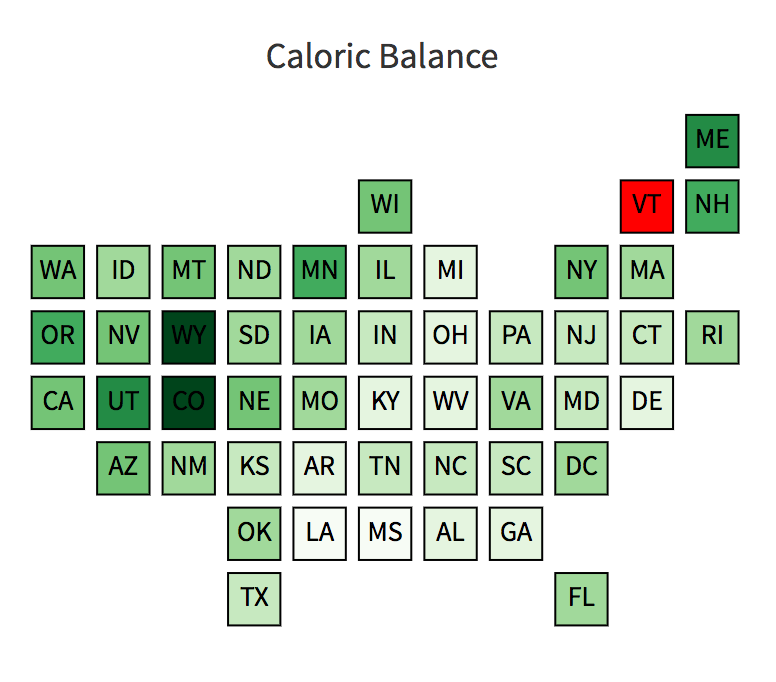
\includegraphics[width=0.6\textwidth]{figures/panometer-map.png}
  \caption[]{
    Lexicocalorimeter map, using square states to control for the disproportionate area and population of US States.
    Here, Vermont is highlighted by a hover.
      }
  \label{fig:panometer-001}
\end{figure}

\begin{figure}[ht]
  \centering
  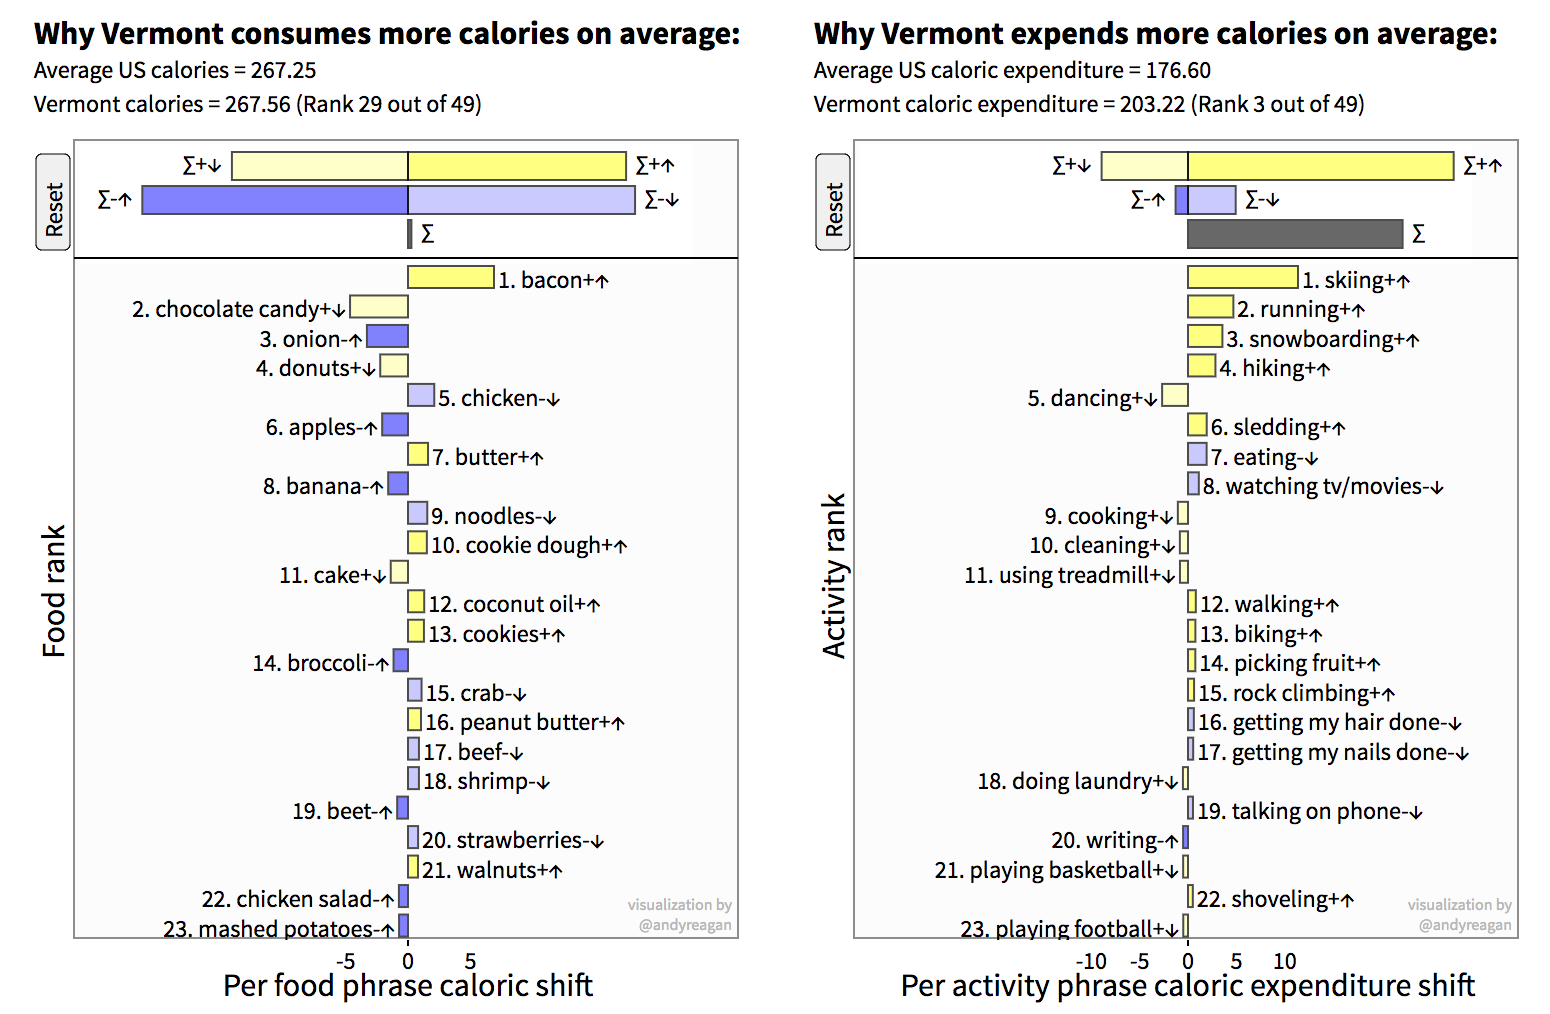
\includegraphics[width=0.9\textwidth]{figures/panometer-wordshifts.png}
  \caption[]{
    Lexicocalorimeter food and activity shifts.
    Here we see which foods and which activities contribute to Vermont's difference in caloric intake and expenditure from the US as a whole.
    We see that Bacon contributes most to caloric intake in Vermont relative to the average US intake, and overall Vermont is a middle-of-the-pack state (29th out of 49).
    On the right, Tweets from Vermont expend more calories than the US average with activities such as skiing, running, snowboarding, hiking, and sledding, giving the outdoorsy Vermont Twitter population the 3rd highest expenditure.
      }
  \label{fig:panometer-002}
\end{figure}

\begin{figure}[ht]
  \centering
  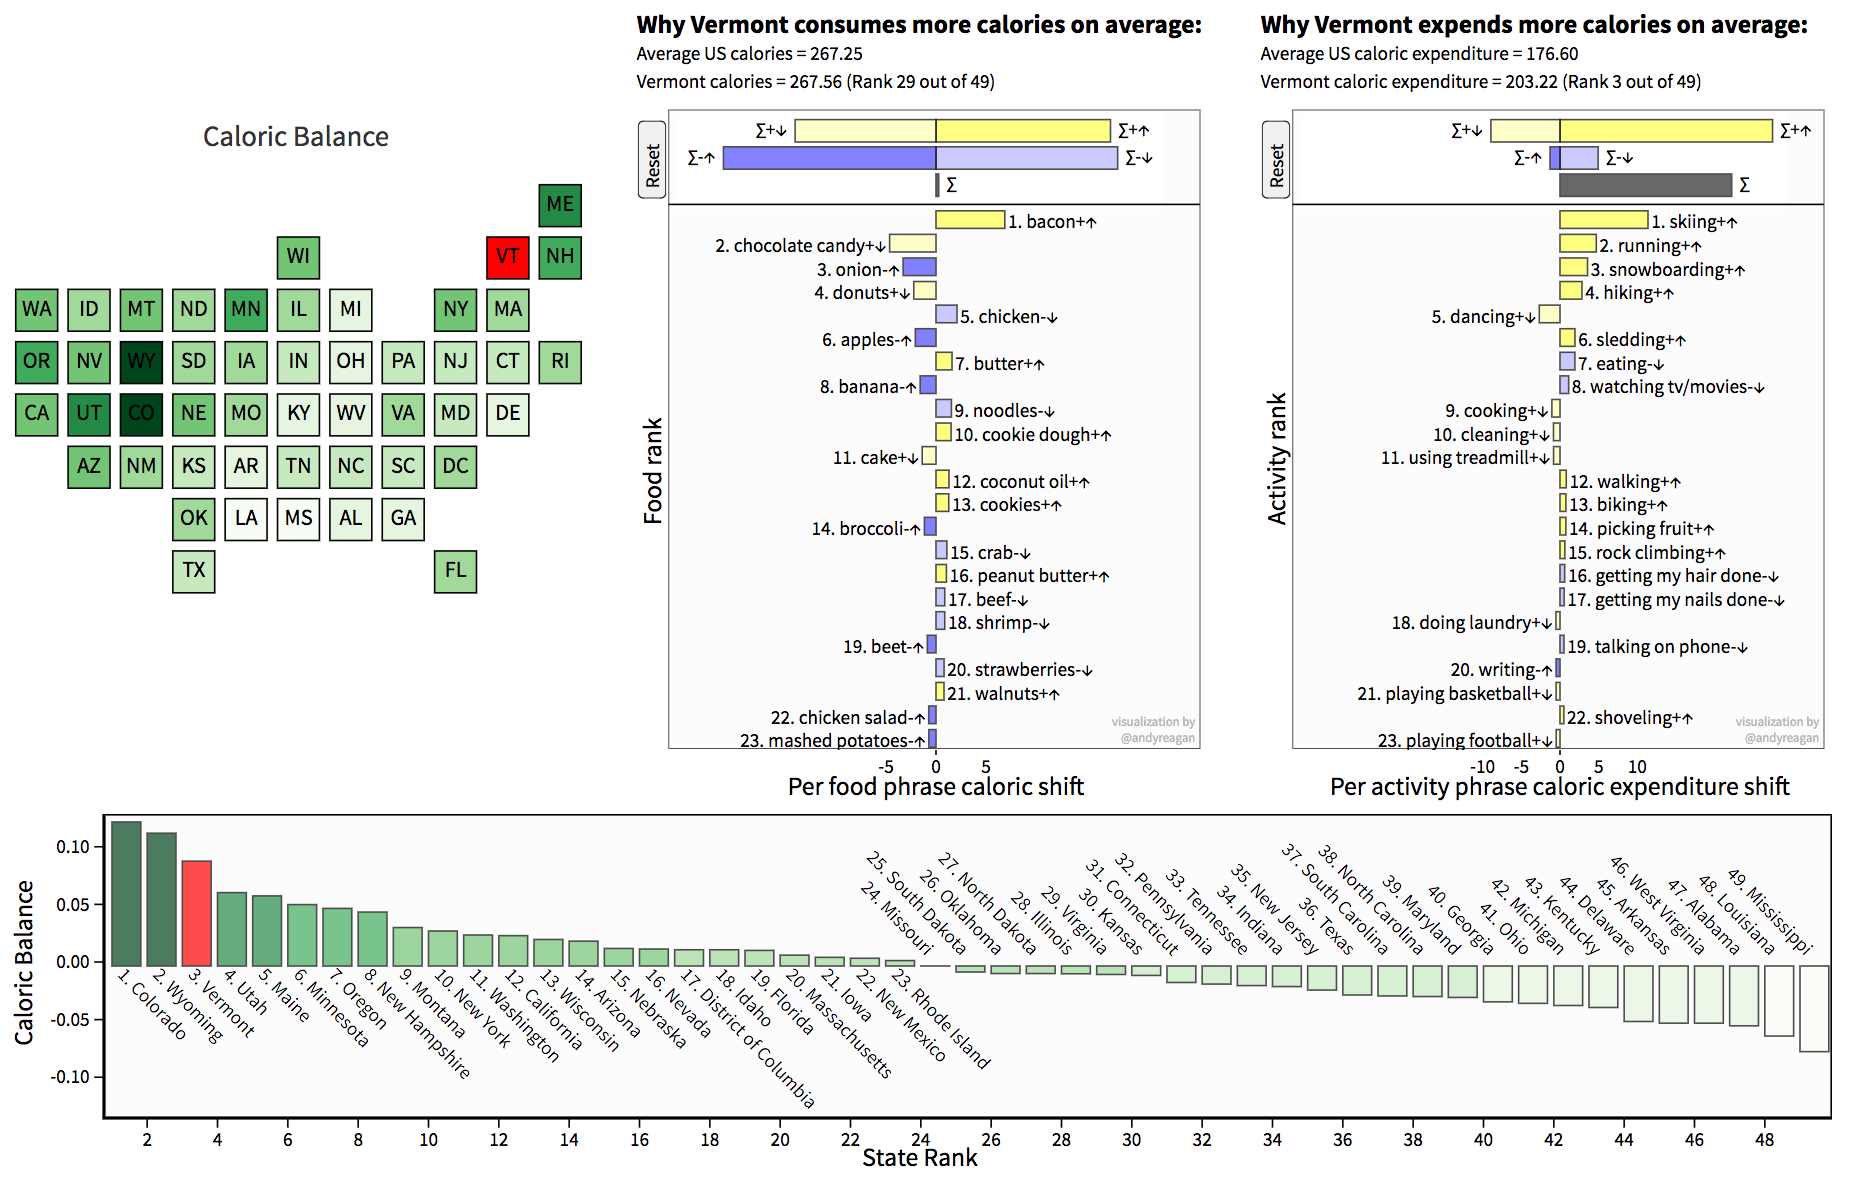
\includegraphics[width=0.9\textwidth]{figures/panometer-overview.png}
  \caption[]{
    Overview of the Lexicocalorimeter dashboard.
    Each view is linked by hovering, and we can explore details of the caloric difference balances between states.
      }
  \label{fig:panometer-003}
\end{figure}

\begin{figure}[ht]
  \centering
  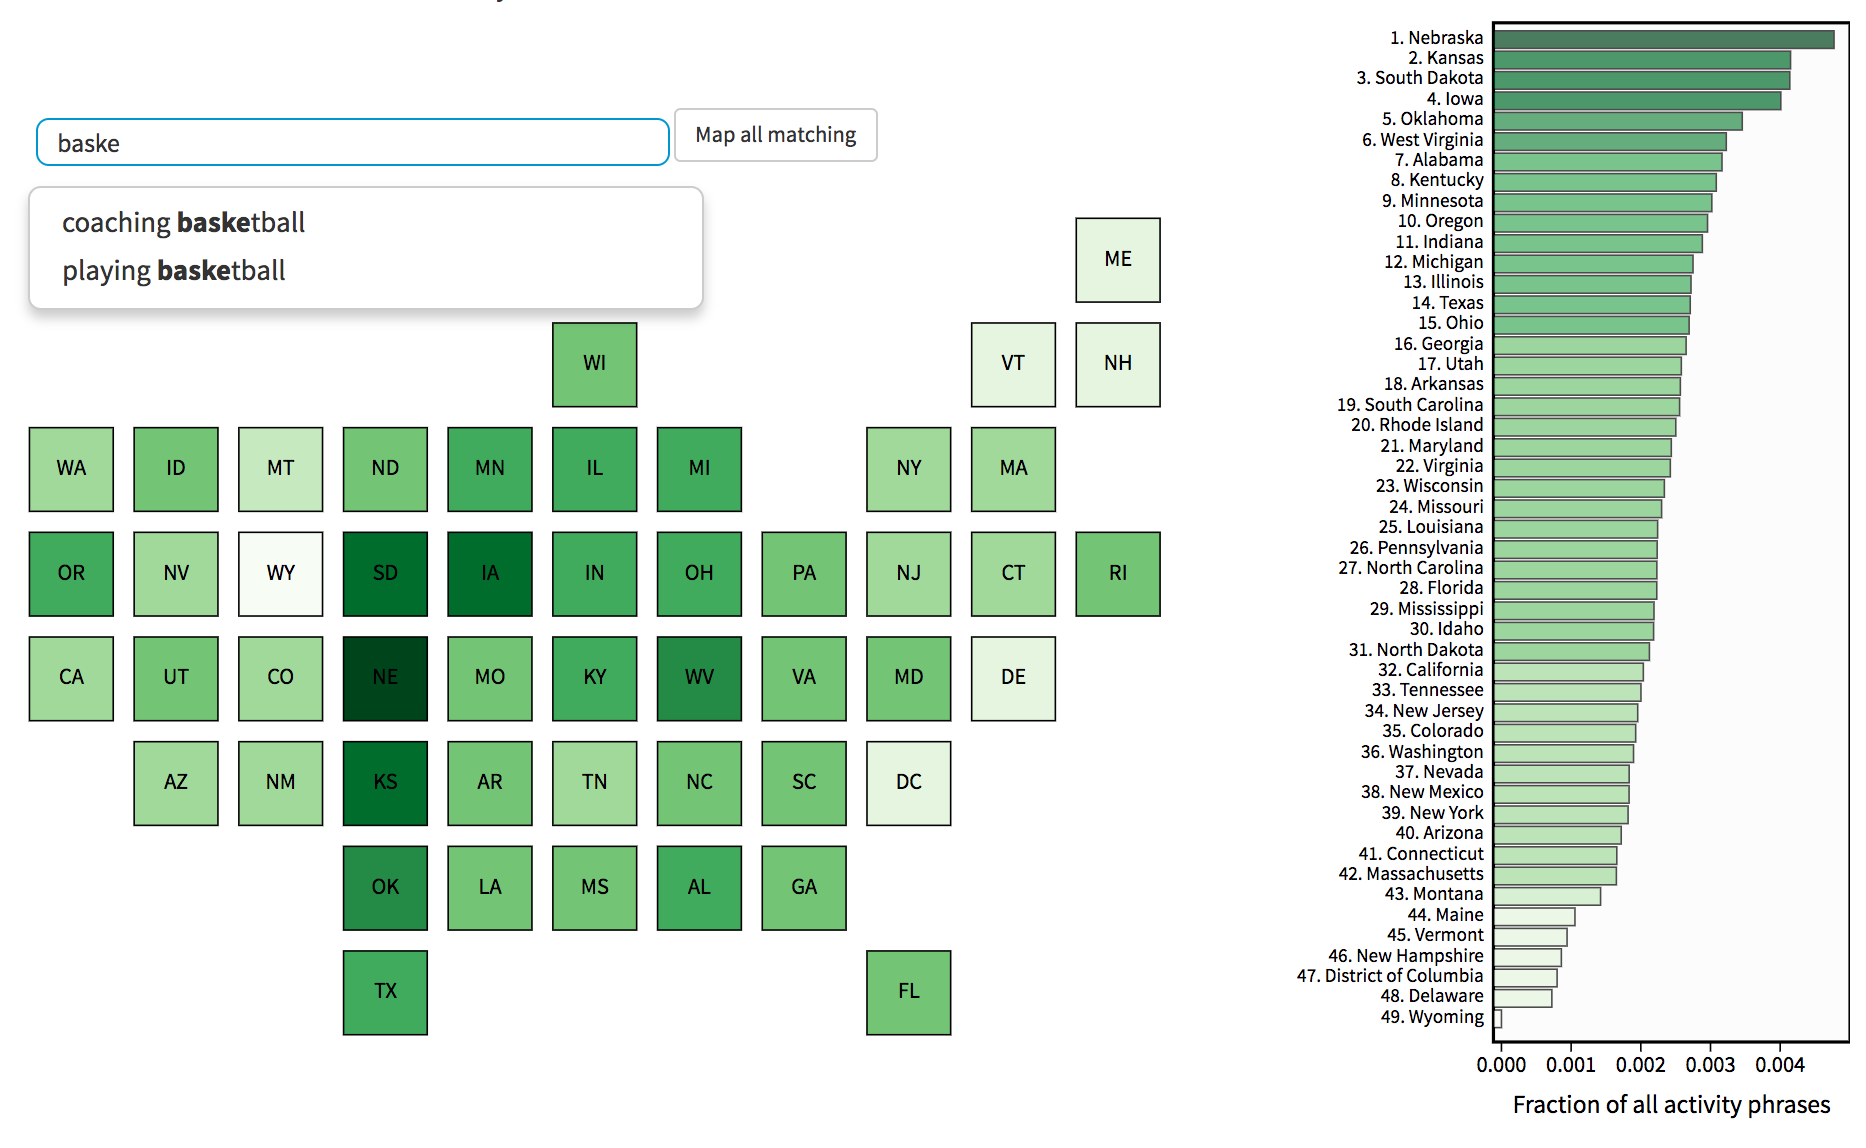
\includegraphics[width=0.9\textwidth]{figures/panometer-activitysearch.png}
  \caption[]{
    Snapshot of the Lexicocalorimeter activity search page.
    A similar page exists for foods.
    Here, we submit the query for ``basketball'', seeing that Nebraskans Tweet more about basketball relative to other activities than other US States.
      }
  \label{fig:panometer-004}
\end{figure}


\clearpage
\pagebreak

\section{Tracking the Teletherms: The spatiotemporal dynamics of the hottest and coldest days of the year}

Paper number eight is
\textit{Tracking the Teletherms: The spatiotemporal dynamics of the hottest and coldest days of the year}
by Peter Sheridan Dodds, Lewis Mitchell, Andrew J. Reagan, and Christopher M. Danforth,
cited as \cite{dodds2016tracking}.
\subsection{Abstract}
\begin{quote}
  Instabilities and long term shifts in seasons,
  whether induced by natural drivers or human activities,
  pose great disruptive threats to ecological, agricultural, and social systems.
  Here, we propose, measure, and explore two fundamental markers of location-sensitive seasonal variations:
  the Summer and Winter Teletherms
  ---
  the on-average annual dates of the hottest and coldest days of the year.
  We analyze daily temperature extremes recorded at 1218 stations across the contiguous United States
  from 1853--2012,
  and observe large regional variation with the Summer Teletherm falling up to 90 days after the Summer Solstice,
  and 50 days for the Winter Teletherm after the Winter Solstice.
  We show that Teletherm temporal dynamics are substantive
  with clear and in some cases dramatic shifts reflective of system bifurcations.
  We also compare recorded daily temperature extremes
  with output from two regional climate models finding considerable though relatively unbiased error.
  Our work demonstrates that Teletherms are an intuitive, powerful, and statistically sound measure
  of local climate change,
  and that they pose detailed, stringent challenges for future theoretical and computational models.
\end{quote}

\subsection{Contribution}

For this paper,
I built the online appendices and transformed the visualizations into online, interactive versions
at \href{http://teletherm.org/}{http://teletherm.org/} using D3 Javascript \citep{bostock2011d3}.
The online appendices are available at \href{http://compstorylab.org/share/papers/dodds2015c/index.html}{http://compstorylab.org/share/papers/dodds2015c/index.html}.
Maps of the United States are shown in Figure \ref{fig:teletherm-map}, with Voronoi cells for each
station colored in addition to the direction and color of the arrows used in
the static maps.
Other features of these online maps include the ability to animate through time,
select a fisheye lens for inspecting the map, and toggle between the various indicators
(Summer/Winter Teletherm day and temperature).

\begin{figure}[tbp!]
  \centering
  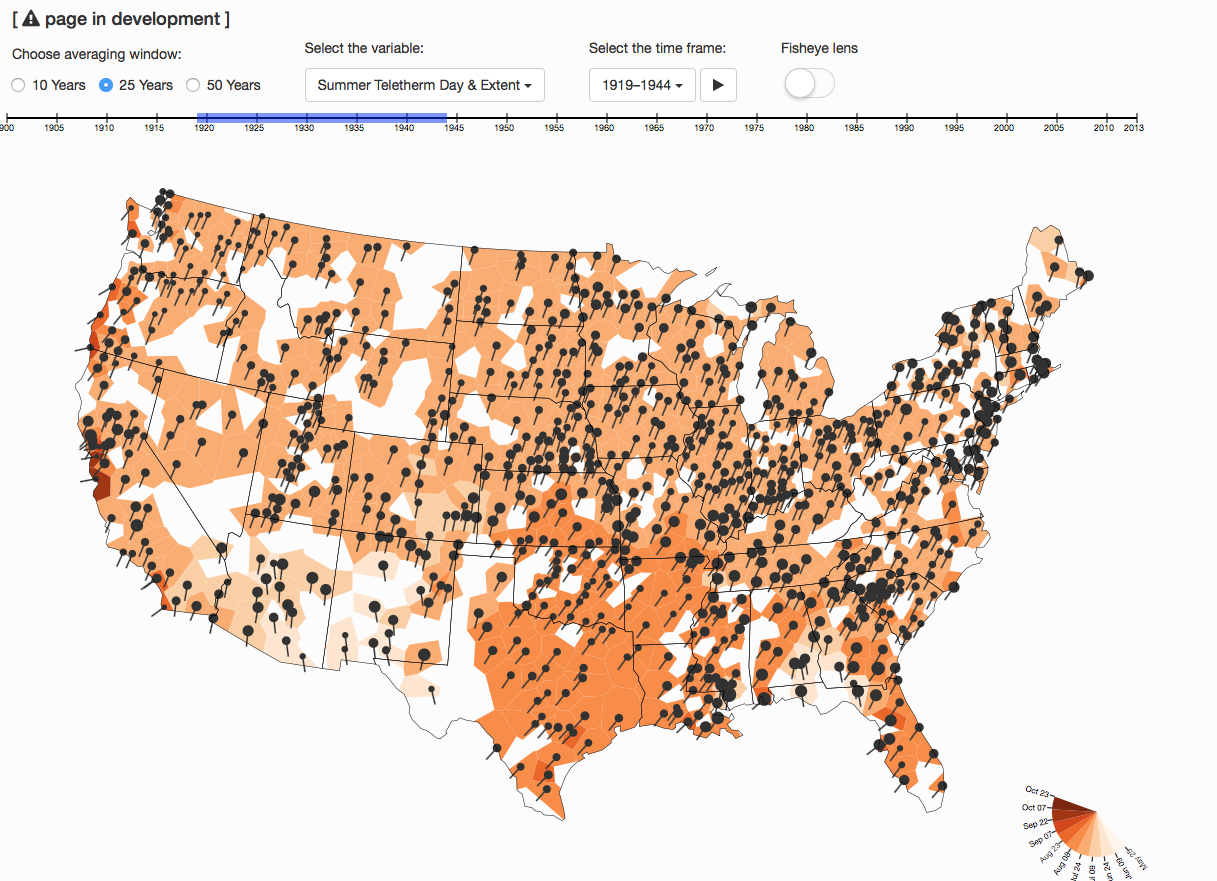
\includegraphics[width=0.96\textwidth]{figures/teletherm-005.png}
  \caption[]{
    Interactive teletherm map with time and variable controls. Select between the teletherm day \& extent and teletherm temperature, the averaging window to compute the teletherms, and the time to show on the map.
    A linear color scale, ``oranges'', is shown for teletherm day and extent.
    A diverging color scale is shown for temperatures, inspired by \href{https://darksky.net}{https://darksky.net}.
    For each weather station, a tooltip hover shows details on demand.
  }
  \label{fig:teletherm-map}
\end{figure}

To realize the goals of this research, the website is designed to communicate
the patterns of Teletherm dynamics at both a local and a regional level.
In addition to building interactive versions of the US maps, I worked with
Professor Dodds to design novel visualizations for the individual station teletherm dynamics.
These plots are shown in Figure \ref{fig:teletherm-splat}, and accompany visualizations of
the time dynamics of Teletherm days, extents, and temperatures.
The online source code repository is publicly available at \href{https://github.com/andyreagan/teletherm.org}{https://github.com/andyreagan/teletherm.org}.

%% The final tool provided at \href{http://teletherm.org/}{http://teletherm.org/} is a

\begin{figure}[tbp!]
  \centering
  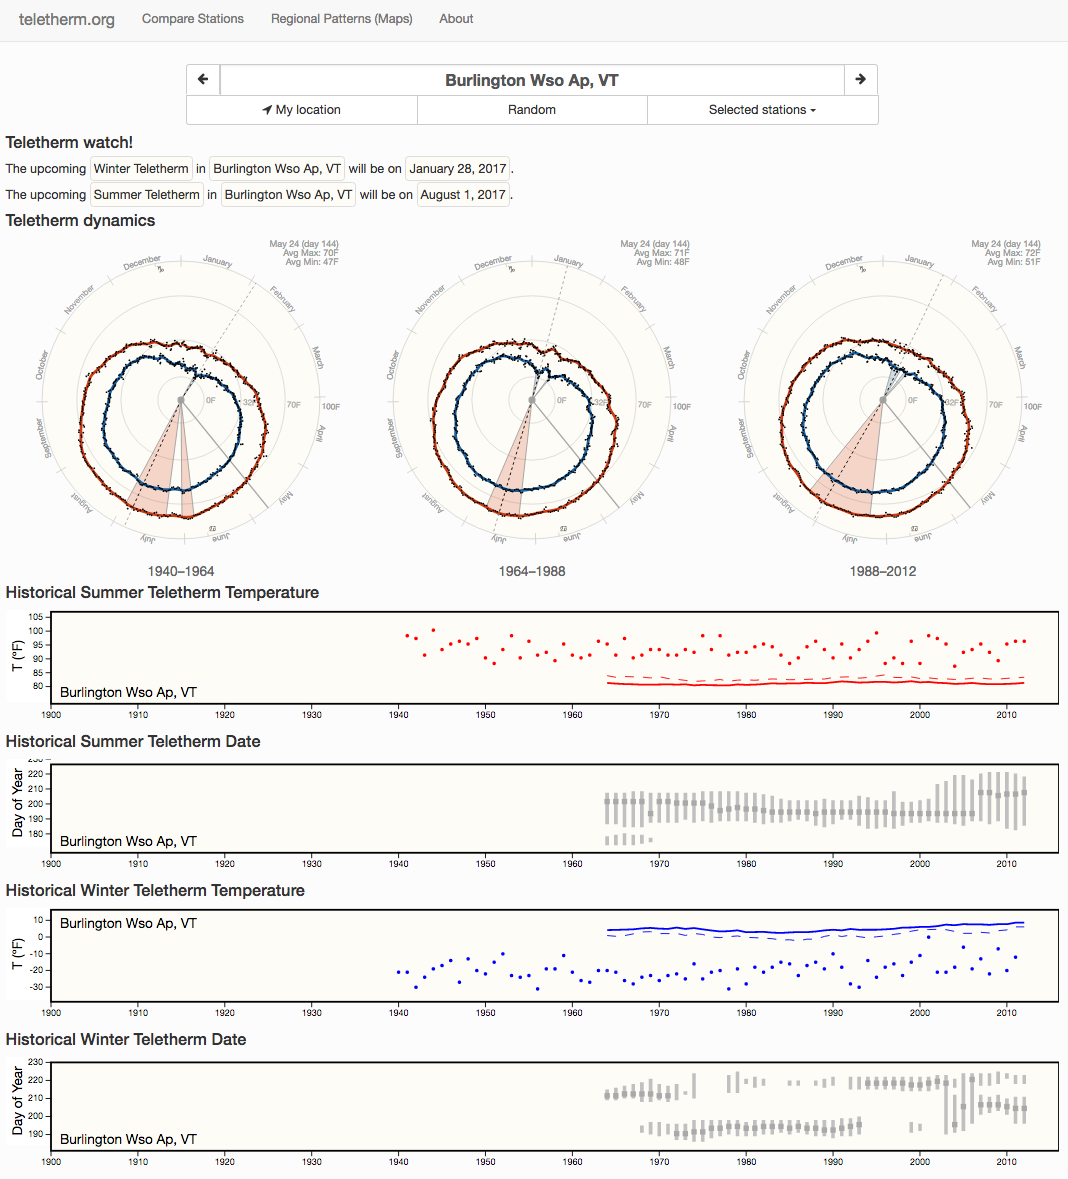
\includegraphics[width=0.96\textwidth]{figures/teletherm-002.png}
  \caption[]{
    Teletherm dials show the yearly temperature dynamics for a single location over a period of time, and time series below show the trends for both temperature extremes and teletherm dates.
    The min and max temperature for each day of the year are smoothed over three 25 year windows, one for each dial, and shown in blue and red, respectively.
    As in the paper, the smoothed temperature is computed with a Gaussian kernel smoothing over the average min/max over days of the year.
    To avoid issues with the boundary, to compute the Gaussian kernel the temperature is wrapped on both ends of the year (with the same data).
    Summer and winter solstice are shown with icons, and the details of the day of year are shown in the upper right of each dial (over which the hover is linked between each dial---they all move together).
  }
  \label{fig:teletherm-splat}
\end{figure}

%% \section{Predicting Flow Reversals in a Computational Fluid Dynamics Simulated Thermosyphon using Data Assimilation}

%% Paper number nine is \textit{Predicting Flow Reversals in a Computational Fluid Dynamics Simulated Thermosyphon using Data Assimilation} by Andrew J. Reagan, Yves Dubief, Peter Sheridan Dodds, and Christopher M. Danforth, cited as \cite{reagan2016predicting}.

%% \subsection{Abstract}
%% \begin{quote}
%%   \input{/Users/andyreagan/projects/2014/11-thermosyphon-paper/paper/thermosyphon-paper.abs.tex}
%% \end{quote}

%% \subsection{Contribution}

%% I wrote the paper, and performed the analysis, working closely with my co-authors.

\clearpage

\section{Divergent Discourse Between Protests and Counter-Protests: \#BlackLivesMatter and \#AllLivesMatter}

Paper number 10 is \textit{Divergent Discourse Between Protests and Counter-Protests: \#BlackLivesMatter and \#AllLivesMatter} by Ryan J. Gallagher, Andrew J. Reagan, Christopher M. Danforth, and Peter Sheridan Dodds, cited as \cite{gallagher2016divergent}.

\subsection{Abstract}

\begin{quote}
  Since the shooting of Black teenager Michael Brown by White police officer Darren Wilson in Ferguson, Missouri,
the protest hashtag \#BlackLivesMatter has amplified critiques of extrajudicial killings of Black Americans.
In response to \#BlackLivesMatter,
other Twitter users have adopted \#AllLivesMatter,
a counter-protest hashtag whose content argues that equal attention should be given to all lives regardless of race.
Through a multi-level analysis,
we study how these protests and counter-protests diverge by quantifying aspects of their discourse.
In particular,
we introduce methodology that not only quantifies these divergences,
but also reveals whether they are from widespread discussion or a few popular retweets within these groups.
We find that \#BlackLivesMatter exhibits many information rich conversations,
while those within \#AllLivesMatter are more muted and susceptible to hijacking.
We also show that the discussion within \#BlackLivesMatter is more likely to center around the deaths of Black Americans,
while that of \#AllLivesMatter is more likely to sympathize with the lives of police officers and express politically conservative views.
\end{quote}

\subsection{Contribution}

My main contribution to this paper was working closely with lead author Ryan Gallagher to collect the data from our Twitter database on the VACC.
We collected data for a number of hashtags, specifically all of the following:

%% \begin{python}
%% keywords = [{"re": re.compile(r"#blacklivesmatter\b",flags=re.IGNORECASE), "folder": "blacklivesmatter",},
%%             {"re": re.compile(r"#alllivesmatter\b",flags=re.IGNORECASE), "folder": "alllivesmatter",},
%%             {"re": re.compile(r"#bluelivesmatter\b",flags=re.IGNORECASE), "folder": "bluelivesmatter",},
%%             {"re": re.compile(r"#policelivesmatter\b",flags=re.IGNORECASE), "folder": "policelivesmatter",},
%%             {"re": re.compile(r"#michaelbrown\b",flags=re.IGNORECASE), "folder": "michaelbrown",},
%%             {"re": re.compile(r"#ferguson\b",flags=re.IGNORECASE), "folder": "ferguson",},
%%             {"re": re.compile(r"#freddiegray\b",flags=re.IGNORECASE), "folder": "freddiegray",},
%%             {"re": re.compile(r"#ericgarner\b",flags=re.IGNORECASE), "folder": "ericgarner",},
%%             {"re": re.compile(r"#icantbreathe\b",flags=re.IGNORECASE), "folder": "icantbreathe",},
%%             {"re": re.compile(r"#sarahbland\b",flags=re.IGNORECASE), "folder": "sarahbland",},
%%             {"re": re.compile(r"#templeton\b",flags=re.IGNORECASE), "folder": "templeton",},]
%% \end{python}

\begin{python}
keywords = [{"re": re.compile(r"#blacklivesmatter\b",flags=re.IGNORECASE)}},
            {"re": re.compile(r"#alllivesmatter\b",flags=re.IGNORECASE)}},
            {"re": re.compile(r"#bluelivesmatter\b",flags=re.IGNORECASE)},
            {"re": re.compile(r"#policelivesmatter\b",flags=re.IGNORECASE)},
            {"re": re.compile(r"#michaelbrown\b",flags=re.IGNORECASE)},
            {"re": re.compile(r"#ferguson\b",flags=re.IGNORECASE)},
            {"re": re.compile(r"#freddiegray\b",flags=re.IGNORECASE)},
            {"re": re.compile(r"#ericgarner\b",flags=re.IGNORECASE)},
            {"re": re.compile(r"#icantbreathe\b",flags=re.IGNORECASE)},
            {"re": re.compile(r"#sarahbland\b",flags=re.IGNORECASE)},
            {"re": re.compile(r"#templeton\b",flags=re.IGNORECASE)},]
\end{python}

After collecting the Tweets for these hashtags, they were reorganized by user, and then collected into a \verb|sqlite| database using Django, a Python web framework.
This web framework was then used to go back and collect the most recent 3,200 Tweets from each public Twitter account that we had found in our initial search.
The collection ended on Nov 25th, 2015, so these Tweets were the 3,200 most recent as of that date.
From this data, we were able to construct the social networks for analysis of the dynamics of these online communities.
